%===============================================================================
% LaTeX sjabloon voor de bachelorproef toegepaste informatica aan HOGENT
% Meer info op https://github.com/HoGentTIN/latex-hogent-report
%===============================================================================

\documentclass[dutch,dit,thesis]{hogentreport}

% TODO:
% - If necessary, replace the option `dit`' with your own department!
%   Valid entries are dbo, dbt, dgz, dit, dlo, dog, dsa, soa
% - If you write your thesis in English (remark: only possible after getting
%   explicit approval!), remove the option "dutch," or replace with "english".

\usepackage{lipsum} % For blind text, can be removed after adding actual content

%% Pictures to include in the text can be put in the graphics/ folder
\graphicspath{{../graphics/}}

%% For source code highlighting, requires pygments to be installed
%% Compile with the -shell-escape flag!
\usepackage[section]{minted}
%% If you compile with the make_thesis.{bat,sh} script, use the following
%% import instead:
%% \usepackage[section,outputdir=../output]{minted}
\usemintedstyle{solarized-light}
\definecolor{bg}{RGB}{253,246,227} %% Set the background color of the codeframe

%% Change this line to edit the line numbering style:
\renewcommand{\theFancyVerbLine}{\ttfamily\scriptsize\arabic{FancyVerbLine}}

%% Macro definition to load external java source files with \javacode{filename}:
\newmintedfile[javacode]{java}{
    bgcolor=bg,
    fontfamily=tt,
    linenos=true,
    numberblanklines=true,
    numbersep=5pt,
    gobble=0,
    framesep=2mm,
    funcnamehighlighting=true,
    tabsize=4,
    obeytabs=false,
    breaklines=true,
    mathescape=false
    samepage=false,
    showspaces=false,
    showtabs =false,
    texcl=false,
}

% Other packages not already included can be imported here

%%---------- Document metadata -------------------------------------------------
% TODO: Replace this with your own information
\author{Arthur Uydens}
\supervisor{Dhr. J. Claes}
\cosupervisor{Dhr. P. Baeke}
\title{Itineris - Ontwikkeling van een AI assistent voor Itineris: technologieën en valkuilen, Arthur Uydens (2024)}
\academicyear{\advance\year by -1 \the\year--\advance\year by 1 \the\year}
\examperiod{1}
\degreesought{\IfLanguageName{dutch}{Professionele bachelor in de toegepaste informatica}{Bachelor of applied computer science}}
\partialthesis{false} %% To display 'in partial fulfilment'
%\institution{Internshipcompany BVBA.}

%% Add global exceptions to the hyphenation here
\hyphenation{back-slash}

%% The bibliography (style and settings are  found in hogentthesis.cls)
\addbibresource{BachelorproefSources.bib}            %% Bibliography file
\defbibheading{bibempty}{}

%% Prevent empty pages for right-handed chapter starts in twoside mode
\renewcommand{\cleardoublepage}{\clearpage}

\renewcommand{\arraystretch}{1.2}

%% Content starts here.
\begin{document}

%---------- Front matter -------------------------------------------------------

\frontmatter

\hypersetup{pageanchor=false} %% Disable page numbering references
%% Render a Dutch outer title page if the main language is English
\IfLanguageName{english}{%
    %% If necessary, information can be changed here
    \degreesought{Professionele Bachelor toegepaste informatica}%
    \begin{otherlanguage}{dutch}%
       \maketitle%
    \end{otherlanguage}%
}{}

%% Generates title page content
\maketitle
\hypersetup{pageanchor=true}

%%=============================================================================
%% Voorwoord
%%=============================================================================

\chapter*{\IfLanguageName{dutch}{Woord vooraf}{Preface}}%
\label{ch:voorwoord}

%% TODO:
%% Het voorwoord is het enige deel van de bachelorproef waar je vanuit je
%% eigen standpunt (``ik-vorm'') mag schrijven. Je kan hier bv. motiveren
%% waarom jij het onderwerp wil bespreken.
%% Vergeet ook niet te bedanken wie je geholpen/gesteund/... heeft

Met deze bachelorproef wil ik een goede manier vinden om een chatbot zinvolle antwoorden te laten geven op vragen die over bedrijfsdata gaat met het gebruik van artificiële intelligentie. Ik heb voor deze bachelorproef nog maar weinig onderzoek naar artificiële intelligentie gedaan maar toch is het altijd een onderwerp geweest dat me fascineerde. 
Ik had verschillende bedrijven gestuurd met de vraag of ze een casus hadden waar ik op kon inwerken maar toen ik antwoord kreeg met een onderwerp van Itineris wist ik al relatief snel dat dit was waar ik onderzoek naar wou doen. Daarom wil ik dus zeker mijn co-promotor, Peter Baeke, bedanken voor mij deze kans te geven en wekelijkse ondersteuning te geven waar het kon. Mijn promotor, Jan Claes, Wil ik ook hartelijk bedanken voor altijd snelle feedback te geven en te helpen met vragen die ik had over het verloop van de bachelorproef. Voor mijn meer technische vragen kon ik ook altijd terecht bij Maarten Glas en Tom Uvin die me ook doorheen het verloop feedback hebben gegeven op mijn werk. 
Ik wens u veel leesplezier en hoop dat u iets nuttig kan halen uit deze bachelorproef!



%%=============================================================================
%% Samenvatting
%%=============================================================================

% TODO: De "abstract" of samenvatting is een kernachtige (~ 1 blz. voor een
% thesis) synthese van het document.
%
% Een goede abstract biedt een kernachtig antwoord op volgende vragen:
%
% 1. Waarover gaat de bachelorproef?
% 2. Waarom heb je er over geschreven?
% 3. Hoe heb je het onderzoek uitgevoerd?
% 4. Wat waren de resultaten? Wat blijkt uit je onderzoek?
% 5. Wat betekenen je resultaten? Wat is de relevantie voor het werkveld?
%
% Daarom bestaat een abstract uit volgende componenten:
%
% - inleiding + kaderen thema
% - probleemstelling
% - (centrale) onderzoeksvraag
% - onderzoeksdoelstelling
% - methodologie
% - resultaten (beperk tot de belangrijkste, relevant voor de onderzoeksvraag)
% - conclusies, aanbevelingen, beperkingen
%
% LET OP! Een samenvatting is GEEN voorwoord!

%%---------- Nederlandse samenvatting -----------------------------------------
%
% TODO: Als je je bachelorproef in het Engels schrijft, moet je eerst een
% Nederlandse samenvatting invoegen. Haal daarvoor onderstaande code uit
% commentaar.
% Wie zijn bachelorproef in het Nederlands schrijft, kan dit negeren, de inhoud
% wordt niet in het document ingevoegd.

\IfLanguageName{english}{%
\selectlanguage{dutch}
\chapter*{Samenvatting}
\lipsum[1-4]
\selectlanguage{english}
}{}

%%---------- Samenvatting -----------------------------------------------------
% De samenvatting in de hoofdtaal van het document

\chapter*{\IfLanguageName{dutch}{Samenvatting}{Abstract}}

\lipsum[1-4]


%---------- Inhoud, lijst figuren, ... -----------------------------------------

\tableofcontents

% In a list of figures, the complete caption will be included. To prevent this,
% ALWAYS add a short description in the caption!
%
%  \caption[short description]{elaborate description}
%
% If you do, only the short description will be used in the list of figures

\listoffigures

% If you included tables and/or source code listings, uncomment the appropriate
% lines.
%\listoftables
%\listoflistings

% Als je een lijst van afkortingen of termen wil toevoegen, dan hoort die
% hier thuis. Gebruik bijvoorbeeld de ``glossaries'' package.
% https://www.overleaf.com/learn/latex/Glossaries

%---------- Kern ---------------------------------------------------------------

\mainmatter{}

% De eerste hoofdstukken van een bachelorproef zijn meestal een inleiding op
% het onderwerp, literatuurstudie en verantwoording methodologie.
% Aarzel niet om een meer beschrijvende titel aan deze hoofdstukken te geven of
% om bijvoorbeeld de inleiding en/of stand van zaken over meerdere hoofdstukken
% te verspreiden!

%%=============================================================================
%% Inleiding
%%=============================================================================

\chapter{\IfLanguageName{dutch}{Inleiding}{Introduction}}%
\label{ch:inleiding}

Het onderzoeks-domein van artificiële intelligentie is in de laatste jaren op een stroomversnelling geraakt en is in korte tijd voor iedereen met internet toegang en een computer toegankelijk geworden. Deze ontwikkeling is dan ook duidelijk te zichtbaar op de bedrijfswereld zoals blijkt uit de resultaten van een  enquête over het gebruik van ICT en e-commerce in bedrijven uitgevoerd door Statbel, het Belgische statistiekbureau. Uit deze enquête blijkt dat bijna een op de zeven bedrijven gebruik maakt van artificiële intelligentie. Bij de bedrijven die meer dan 250 werknemers hebben komt dit aan een op de twee bedrijven. ~\autocite{STATBEL2023}
Deze bachelorproef kijkt naar het ontwikkelen van een chatbot die kan antwoorden op vragen die te maken hebben met losse data die op verschillende webapplicaties staan. 


\section{\IfLanguageName{dutch}{Probleemstelling}{Problem Statement}}%
\label{sec:probleemstelling}

Itineris bied software aan voor je nutsvoorzieningen zoals water of elektriciteit te beheren. Ze bieden hier ook customer service voor aan maar vaak als er een vraag gesteld wordt of er een probleem wordt vastgesteld moeten de medewerkers op meerdere webpagina's of webapplicaties de data gaan bekijken/vergelijken om vast te stellen wat er aan de hand is. Dit neemt tijd in beslag en ze kunnen soms dingen over het hoofd zien. 

\section{\IfLanguageName{dutch}{Onderzoeksvraag}{Research question}}%
\label{sec:onderzoeksvraag}

Hoe kunnen we de efficiënte ontwikkeling van een co-pilot bevorderen door het identificeren van verschillende valkuilen en technologieën met specifieke aandacht voor de vereisten van de onderneming? 

\section{\IfLanguageName{dutch}{Onderzoeksdoelstelling}{Research objective}}%
\label{sec:onderzoeksdoelstelling}

Het onderzoek moet een oog geven op de ontwikkeling van een chatbot en welke technologieën hierbij te pas komen. Een proof of concept wordt hierbij opgesteld om de keuze van de technologieën toe te lichten. 


\section{\IfLanguageName{dutch}{Opzet van deze bachelorproef}{Structure of this bachelor thesis}}%
\label{sec:opzet-bachelorproef}

% Het is gebruikelijk aan het einde van de inleiding een overzicht te
% geven van de opbouw van de rest van de tekst. Deze sectie bevat al een aanzet
% die je kan aanvullen/aanpassen in functie van je eigen tekst.

De rest van deze bachelorproef is als volgt opgebouwd:

In Hoofdstuk~\ref{ch:stand-van-zaken} wordt een overzicht gegeven van de stand van zaken binnen het onderzoeksdomein, op basis van een literatuurstudie.

In Hoofdstuk~\ref{ch:methodologie} wordt de methodologie toegelicht en worden de gebruikte onderzoekstechnieken besproken om een antwoord te kunnen formuleren op de onderzoeksvragen.

% TODO: Vul hier aan voor je eigen hoofstukken, één of twee zinnen per hoofdstuk

In Hoofdstuk~\ref{ch:conclusie}, tenslotte, wordt de conclusie gegeven en een antwoord geformuleerd op de onderzoeksvragen. Daarbij wordt ook een aanzet gegeven voor toekomstig onderzoek binnen dit domein.
\chapter{\IfLanguageName{dutch}{Stand van zaken}{State of the art}}%
\label{ch:stand-van-zaken}

% Tip: Begin elk hoofdstuk met een paragraaf inleiding die beschrijft hoe
% dit hoofdstuk past binnen het geheel van de bachelorproef. Geef in het
% bijzonder aan wat de link is met het vorige en volgende hoofdstuk.

% Pas na deze inleidende paragraaf komt de eerste sectiehoofding.

%Dit hoofdstuk bevat je literatuurstudie. De inhoud gaat verder op de inleiding, maar zal het onderwerp van de bachelorproef *diepgaand* uitspitten. De bedoeling is dat de lezer na lezing van dit hoofdstuk helemaal op de hoogte is van de huidige stand van zaken (state-of-the-art) in het onderzoeksdomein. Iemand die niet vertrouwd is met het onderwerp, weet nu voldoende om de rest van het verhaal te kunnen volgen, zonder dat die er nog andere informatie moet over opzoeken \autocite{Pollefliet2011}.
%
%Je verwijst bij elke bewering die je doet, vakterm die je introduceert, enz.\ naar je bronnen. In \LaTeX{} kan dat met het commando \texttt{$\backslash${textcite\{\}}} of \texttt{$\backslash${autocite\{\}}}. Als argument van het commando geef je de ``sleutel'' van een ``record'' in een bibliografische databank in het Bib\LaTeX{}-formaat (een tekstbestand). Als je expliciet naar de auteur verwijst in de zin (narratieve referentie), gebruik je \texttt{$\backslash${}textcite\{\}}. Soms is de auteursnaam niet expliciet een onderdeel van de zin, dan gebruik je \texttt{$\backslash${}autocite\{\}} (referentie tussen haakjes). Dit gebruik je bv.~bij een citaat, of om in het bijschrift van een overgenomen afbeelding, broncode, tabel, enz. te verwijzen naar de bron. In de volgende paragraaf een voorbeeld van elk.
%
%\textcite{Knuth1998} schreef een van de standaardwerken over sorteer- en zoekalgoritmen. Experten zijn het erover eens dat cloud computing een interessante opportuniteit vormen, zowel voor gebruikers als voor dienstverleners op vlak van informatietechnologie~\autocite{Creeger2009}.
%
%Let er ook op: het \texttt{cite}-commando voor de punt, dus binnen de zin. Je verwijst meteen naar een bron in de eerste zin die erop gebaseerd is, dus niet pas op het einde van een paragraaf.


Om te weten welke technologieën we van de artificiële intelligentie kunnen gebruiken voor onze chatbot moeten we eerst het begrip artificiële technologie en toepasselijke technologieën onder deze wetenschap bekijken. Zo is artificiële intelligentie simpel gezegd een algoritme dat intelligentie probeert na te bootsen om bepaalde taken uit te voeren. De effectieve implementaties van artificiële intelligentie kunnen op vele verschillende manieren voorkomen, de nodige gaan we hieronder overlopen. 

\section{Artificiële intelligentie (AI)}
Artificiële intelligentie, of AI, is technologie dat toelaat om met computers en machines probleem oplossend te denken en menselijke intelligentie na te bootsen~\autocite{IBMc}. Artificiële intelligentie heeft veel toepassingen en daardoor is het ook een onderwerp dat we steeds vaker verwerken. 
Dit kan op vele manieren gebeuren en eigenlijk is dit een koepelterm voor meerdere specifieke technologieën (zie onderstaande mind map op figuur \ref{fig:mindmap}). De verschillende sub-onderwerpen en bepaalde toepassingen hiervan zijn: 

\begin{itemize}
    \item Machine Learning (ML): Wordt gebruikt bij toepassingen zoals zelfrijdende auto's.
    \item Natural Language Processing (NLP): Wordt gebruikt voor software die met talen werkt zoals Google translate.
    \item Speech: Wordt gebruikt voor toepassingen zoals Alexa of Siri.
    \item Expert Systems: Computer programma's die zich kan voordoen als een expert van een vakgebied om oordelen te maken. 
    \item Planning, scheduling and optimization: Software om takenvolgorde, toewijzing van middelen en time management.  
    \item Robotics: Het besturen van robots/machines. 
    \item Vision: Beeldherkenning zoals de face recognition op een smartphone.
\end{itemize}


\begin{figure}
    \centering
    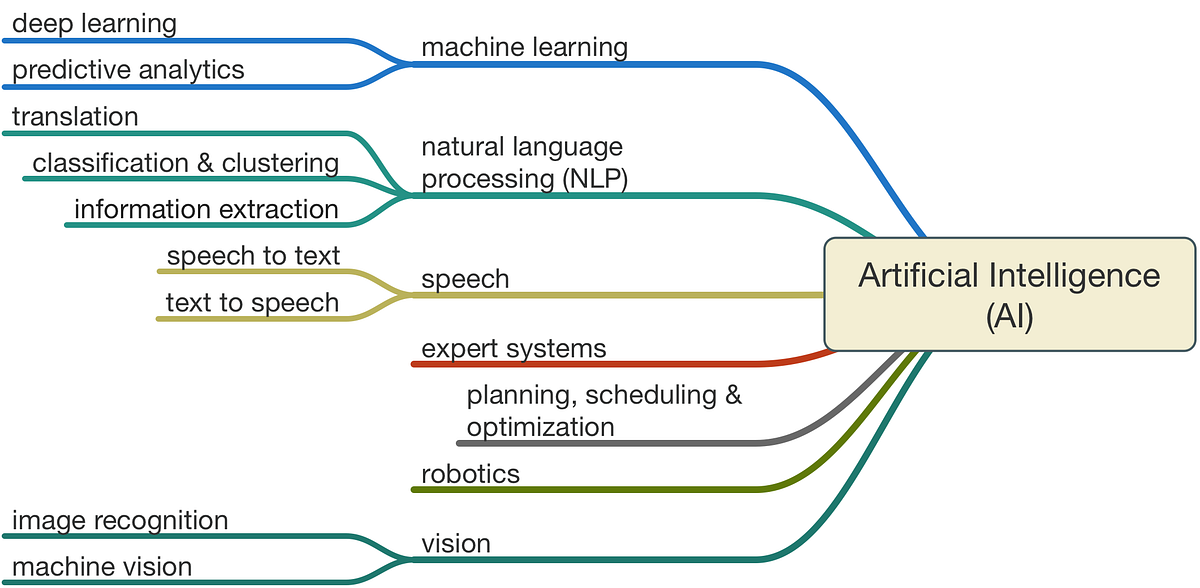
\includegraphics[width=0.75\textwidth]{mindmapai}
    \caption{Mind map van Artificiële Intelligentie}
    \label{fig:mindmap}
\end{figure}

Deze technologieën staan niet altijd los van elkaar, zo kan het zijn dat de ene technologie gebruik maakt van algoritmes uit een andere technologie. 

\subsection{Geschiedenis}
Het onderzoeksdomein van artificiële intelligentie is al een stuk langer aanwezig dan wat de meeste mensen denken. Volgens een artikel van ~\textcite{Europe} is het nog steeds een relatief “jong” onderzoeksdomein van 60 jaar oud terwijl de meeste mensen er maar in contact mee zijn gekomen de laatste 10 jaren.  Geïnstantieerd in de tweede wereldoorlog, is de ontwikkeling sterk gelinkt aan die van computers en heeft geleid naar de mogelijkheid om computers steeds ingewikkeldere taken te laten uitvoeren, wat we hiervoor enkel aan mensen konden overlaten~\autocite{Europe}.

\section{Natural Language Processing (NLP)}
Natuurlijke taalverwerking, of NLP, combineert computationele taalkunde (op regels gebaseerde modellering van menselijke taal) met statistische en machine learning-modellen om computers en digitale apparaten in staat te stellen tekst en spraak te herkennen, begrijpen en genereren~\autocite{IBMa}. Tegenwoordig hebben de meeste mensen hier al contact mee gehad in de vorm van een chatbot, een vertaal assistent of dergelijke. Maar Natural Language Processing speelt ook een steeds belangrijkere rol in bedrijfsoplossingen die helpen om de werklast van de medewerkers te verminderen en de productiviteit een boost te geven. Aangezien Natural Language Processing instaat voor computers het vermogen te geven van tekst en gesproken taal te begrijpen is het ook deel van wat vaak de drie pillaren van conversationele AI wordt genoemd. 

Deze pilaren zijn: 
\begin{itemize}
    \item Natural Language Processing 
    \item Natural Language Understanding
    \item Natural Language Generation
\end{itemize}
Deze pilaren hebben elk hun eigen functie en eigen werking maar bouwen allemaal op elkaar om een conversatie tot stand te kunnen brengen. Het weglaten van een van de drie pilaren zou dus zorgen voor een verminderde kwaliteit. 

\subsection{Natural Language Understanding (NLU)}
De menselijke taal is heel ingewikkeld en zonder de mogelijkheid voor bepaald stukken tekst te interpreteren kan je soms belangrijke informatie niet bekomen. Natural Language Understanding (NLU) is een cruciaal aspect van de verwerking van natuurlijke taal, waarbij gebruik wordt gemaakt van vooraf getrainde taalmodellen (PLM's) voor representatie~\autocite{LvxiaoweiXu2023}. NLU omvat het extraheren en weergeven van de betekenis van teksten en dialogen, waarbij ervoor wordt gezorgd dat de interpretatie in lijn is met de bedoelde boodschap van de spreker voor latere redenering en actie bij kunstmatige intelligente agents. Ondanks de vooruitgang blijft het debat over het vermogen van NLU-systemen om de ware taal te begrijpen bestaan, met discussies over de noodzaak van gestructureerde kennisintegratie om interpretatieve en inferentiële vaardigheden te verbeteren . NLU-systemen zijn bedoeld om de kloof tussen computationele modellen en menselijke taalverwerking te overbruggen, waarbij wordt gestreefd naar alomvattend taalbegrip en -generatie binnen intelligente agenten.


\subsection{Natural Language Generation (NLG)}
Eens een computer in staat is van te zien wat er precies in een tekst gezegd is en wat er mee bedoeld wordt zal de computer ook een nuttig antwoord of actie moeten weerleggen. Hiervoor wordt er gebruik gemaakt van Natural Language Generation, NLG is een proces waarbij computersystemen op basis van bepaalde informatie verstaanbare teksten genereren in menselijke taal ~\autocite{Yang2022}. NLG heeft aanzienlijke vooruitgang geboekt dankzij Artificiële Intelligentie, waaronder deep-learning-algoritmen en neurale netwerken. NLG omvat het creëren van tekst die bepaalde informatie nauwkeurig weergeeft, grammaticaal correct is en voldoet aan specifieke criteria. Het speelt een rol in verschillende sectoren, zoals business intelligence, klantenservice, gezondheidszorg, onderwijs en cyberbeveiliging, en verbetert de communicatie- en besluitvormingsprocessen~\autocite{Woo}. NLG-tools zijn in onderwijsomgevingen gebruikt om de schrijfkwaliteit van studenten te analyseren, wat aantoont dat meer geavanceerde strategieën in de interactie met NLG-tools leiden tot betere menselijke beoordelingen voor gegenereerde inhoud. Over het algemeen is NLG een essentieel onderdeel van kunstmatige intelligentie, dat het mogelijk maakt om coherente en zinvolle menselijke taal te genereren op basis van gestructureerde gegevens.

\section{Transformers}
Transformers zijn geïntroduceerd in 2017 door Google en sinds dan is er een explosie geweest in het aantal geavanceerde modellen (die gerelateerd zijn aan de transformer architectuur) die ontwikkeld werden en het gebruik van deze modellen heeft het belang van Natural Language Processing nog versterkt ~\autocite{Suresh2022}.  Deze modellen hebben de manier veranderd waarop we menselijke taal verwerken en begrijpen, waardoor de grenzen van machinaal leren worden verlegd en opmerkelijke vooruitgang in verschillende NLP-taken mogelijk wordt gemaakt. Van automatische vertaling tot het beantwoorden van vragen en het samenvatten van teksten: Transformers zijn dé architectuur geworden, die ongekende prestatieniveaus laat zien~\autocite{Nemeon}. 
Transformer-modellen vertrouwen op zelfaandachtsmechanismen, waardoor ze sneller kunnen leren dan traditionele modellen, zoals modellen voor het lange kortetermijngeheugen (LSTM). Een zelfaandachtig transformatormodel kan naar verschillende delen van een reeks, of de gehele context van een zin, kijken om voorspellingen te genereren.

\subsection{Embeddings}
De ruwe tekstdata die we hebben, kan niet worden gebruikt om transformer-modellen te trainen omdat ze enkel getallen begrijpen. Er werden eerder al bewerkingen gebruikt om dingen uit de teksten te halen maar er was er nog geen die de tekst kon coderen in getallen. Embeddings was de eerste manier om begrijpelijke informatie in die getallen te coderen, of de juiste manier van zeggen zou vectoren zijn. Dus in plaats van de tokens naar de encoder door te geven, worden de embeddings ervan doorgegeven. Maar een groot probleem was het coderen van de informatie over de positie van de woorden in de embeddings. Standaard embedding mapte elk token gewoon naar een n-dimensionale vector, maar codeerde nooit de positie-informatie.
Om de positie-informatie van de tokens te coderen, kan een andere embedding genaamd positionele embedding worden gebruikt. Bij positionele embedding voeden we in plaats van de tokens van de woorden als invoer de positie-ids of indices van elke zin in. Dit maakt het mogelijk voor de positie-embeddinglaag om een nuttige representatie van de posities te geven. De uiteindelijke uitvoer van de embeddingslaag wordt gegenereerd door de token-embeddings en positie-embeddings toe te voegen en een normalisatie toe te passen op het resultaat zodat er geen enorme waarden zijn ~\autocite{Suresh2022}.

\subsection{Zelfaandachtsmechanisme}
De embeddings die naar de Encoder (zie \ref{ssec:Encoder}) worden gestuurd zijn statisch en bevatten een bepaalde hoeveelheid informatie. Het zelfaandachtsmechanisme houdt rekening met de context van de woorden of tokens in een zin en codeert die informatie in hun respectievelijke embeddings. Het coderen van de context in de embeddings is belangrijk omdat homoniemen in een bepaald stuk tekst aan de zelfde embeddings worden toegewezen. Zo zou bijvoorbeeld een bank in de zin van een geldbank dezelfde embeddingwaarde hebben als een bank waarop je gaat zitten in het park. Wanneer de zelfaandachtslaag klaar is met de verkregen embeddings zullen deze woorden hun context gecodeerd hebben. Hiermee kan het model aandachtscores berekenen en op basis hiervan zal het model hogere gewichten toekennen aan tokens die semantisch gerelateerd zijn (een gelijkaardige/ gelinkte betekenis hebben)~\autocite{Suresh2022}. 


\subsection{Encoder} \label{ssec:Encoder}
De encoder is verantwoordelijk voor het verwerken van de invoerreeks bestaande uit embeddings en als output zorgt het voor dezelfde vorm als de input maar nu hebben de embeddings veel contextuele informatie zoals betekenis, positie van het woord, etc... ~\autocite{Suresh2022} . Het bestaat uit een stapel identieke lagen, elke laag bestaat uit een zelfaandachtsmechanisme gevolgd door een feed-forward neuraal netwerk. Het zelfaandachtsmechanisme laat het model concentreren op verschillende delen van de invoerreeks en het feed-forward neuraal netwerk verwerkt de informatie lokaal. Door deze samenwerking worden niet-lineaire transformaties mogelijk gemaakt. 

\subsection{Decoder}
De decoder accepteert de gecodeerde representaties van de encoder en genereert een uitvoerreeks. Het bevat ook zelfaandachtsmechanismen om afhankelijkheden binnen de uitvoerreeks vast te leggen en aandacht te besteden aan de relevante delen van de invoerreeks. Hierdoor kan het model contextueel bewuste uitput genereren voor taken zoals automatische vertaling of samenvatting van teksten. 

\subsection{Architectuur}
Om de transformator modellen te begrijpen is het soms handig van deze visueel voor te stellen zoals op figuur {TODO}. In dit voorbeeld zien we een transformator model met als encoder het BERT model en decoder het GPT model. Het BERT model gebruikt het encoder gedeelte van de transformer architectuur om de semantiek van de tekst te begrijpen. Het GPT model gebruikt dan het decoder gedeelte van het transformer model om tekst te genereren voor de output aan de hand van de doorgegeven input van de encoder~\autocite{Heidloff2023}. 


\begin{figure}
    \centering
    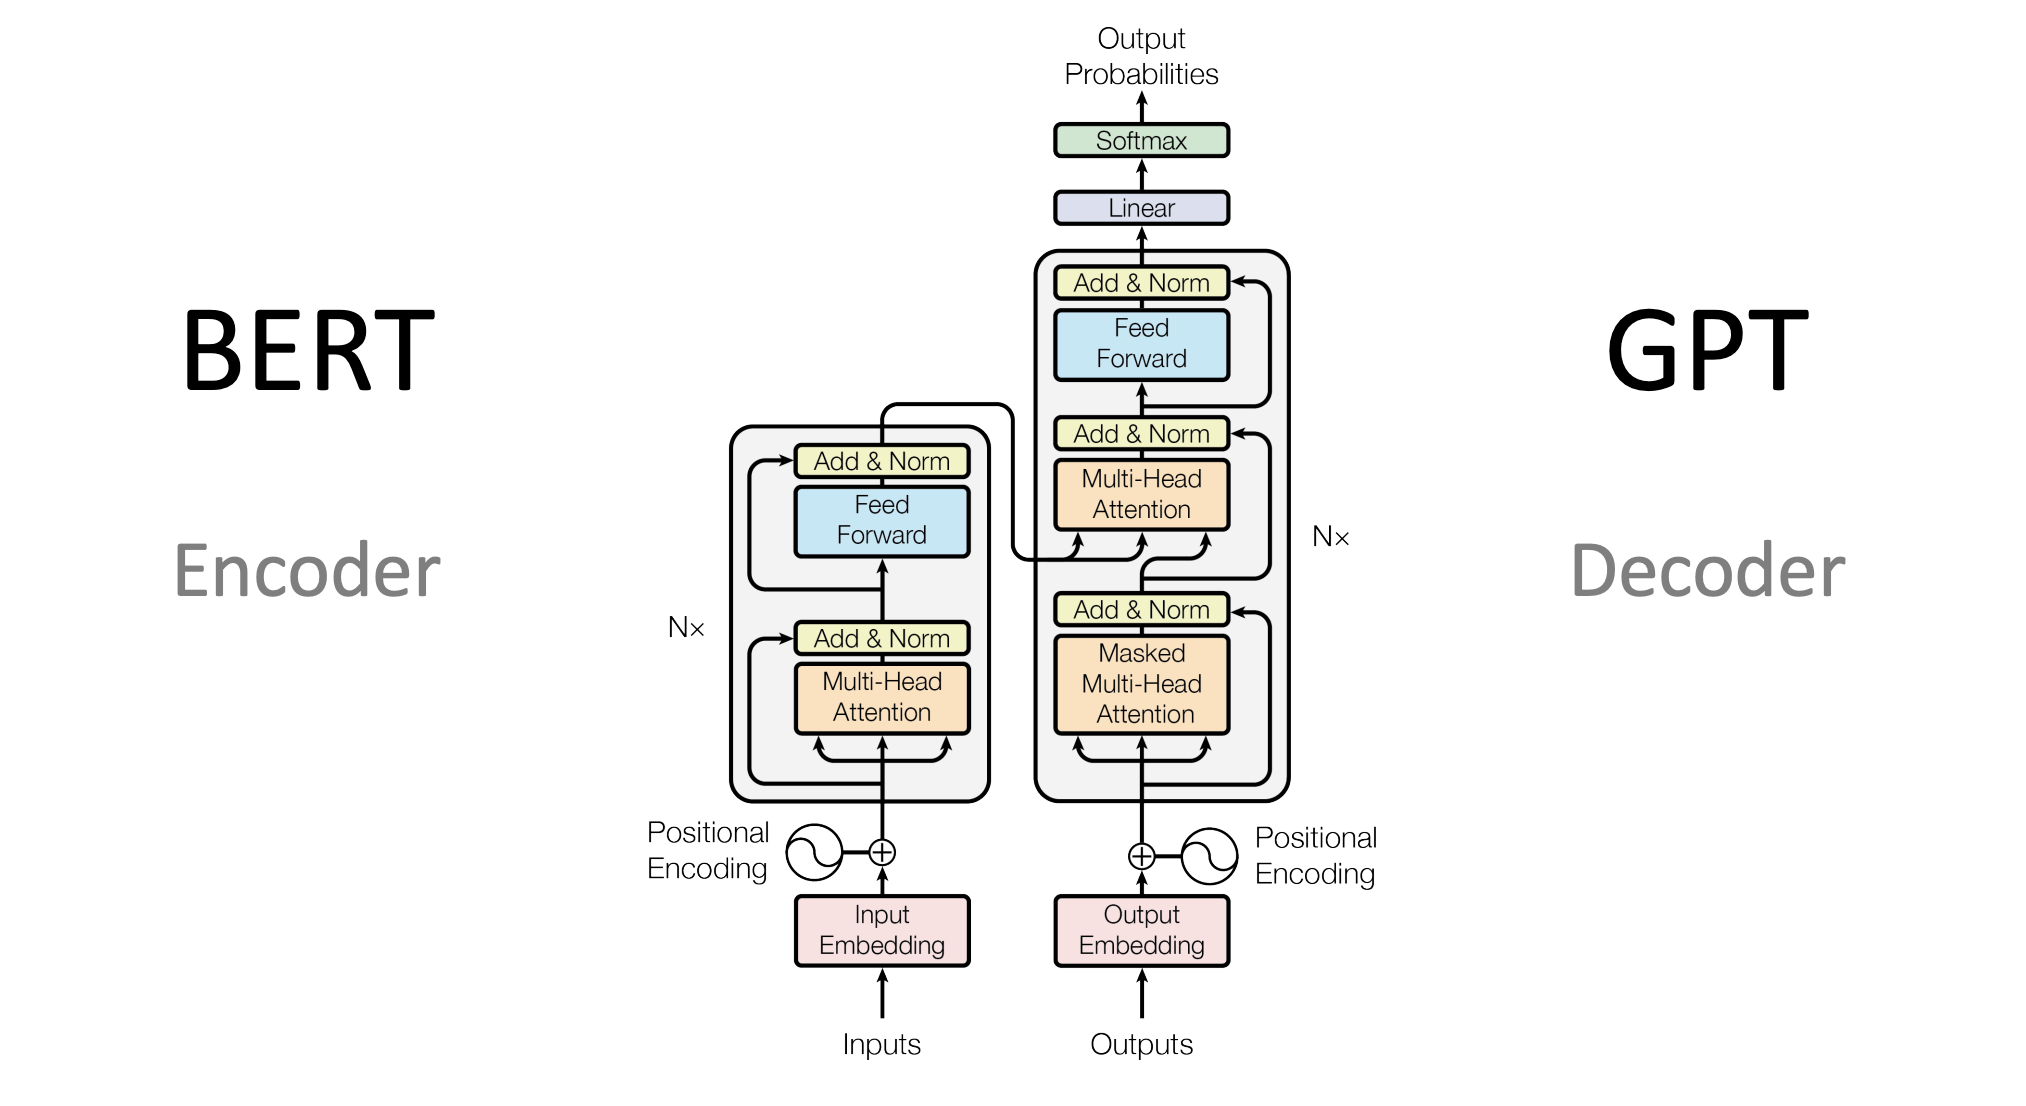
\includegraphics[width=0.75\textwidth]{transformers}
    \caption{Transformer model}
    \label{fig:transformer}
\end{figure}


\section{Large Language Models (LLMs)}
Een Large Language Model (LLM) is een deep learning algoritme dat een reeks natuurlijke taalverwerkingstaken kan uitvoeren.  De modellen maken gebruik van transformator modellen en zijn getraind op grote datasets. Zo kunnen ze teksten of andere content herkennen, vertalen, voorspellen of genereren. Naast het aanleren van menselijke talen aan toepassingen van artificiële intelligentie, kunnen large language models ook getraind worden om verschillende taken uit te voeren, zoals het begrijpen van eiwitstructuren, het schrijven van softwarecode en nog veel meer. 

\subsection{GPT}
Generative Pretrained Transformer modellen zijn taalvoorspellingsmodellen voor algemene doeleinden. Met andere woorden: het zijn computerprogramma's die informatie kunnen analyseren, extraheren, samenvatten en anderszins gebruiken om inhoud te genereren. Generatieve AI technologie is in staat van content te produceren zoals text en fotos waarbij het Pretrained gedeelte betekent dat deze modellen opgeslagen netwerken zijn die al hebben geleerd hoe een bepaalde taak uit te voeren of probleem op te lossen aan de hand van een grote dataset. Deze modellen worden vaak gebruikt in conversationele AI om de User Experience zo persoonlijk en menselijk mogelijk te maken. 
Er bestaan hier vele modellen onder maar hier zal het vooral over de bekende GPT-3 en GPT-4 van OpenAI gaan, wat ook de modellen zijn die gehanteerd zullen worden in de proof-of-concept. 
GPT-3 staat voor "Generative Pre-trained Transformer 3", en het is een geavanceerd AI-model dat is ontwikkeld door OpenAI. Het is het derde model in de reeks van "Transformers" die zijn ontworpen voor natuurlijke taalverwerkingstaken. GPT-3 is getraind op een enorme hoeveelheid tekstgegevens en kan vervolgens worden gebruikt voor verschillende taken, zoals het genereren van tekst, het beantwoorden van vragen en het vertalen van talen. Het model kan opmerkelijk complexe en coherente mensachtige tekst produceren, waardoor het een krachtig instrument is voor een breed scala aan toepassingen, van chatbots tot contentgeneratie~\autocite{Schulze2024}.
GPT-4 is het meest recente model van OpenAI. Het is een groot multimodaal model (LMM), wat betekent dat zowel beeldinvoer als tekst kan worden geparseerd. Deze iteratie is het meest uitgebreide GPT-model, dat prestaties op menselijk niveau laat zien in verschillende benchmarks op professioneel en academisch gebied. Ter vergelijking: GPT-3.5 behaald bij de onderste 10 procent van de deelnemers aan een gesimuleerd staafexamen. GPT-4 scoort in de top 10 procent~\autocite{Schulze2024}.

\section{Chatbots}
Chatbots bestaan onder vele vormen maar ze hebben allemaal ongeveer hetzelfde doel. Simpelweg gezegd is een chatbot een programma dat conversaties tussen mensen nabootst en verwerkt. Dit laat mensen toe om te intrageren met digitale toestellen zoals ze met een echte persoon zouden doen. Deze programma's kunnen heel simpel zijn om simpele korte antwoorden te geven maar ze kunnen ook heel uitgebreid ontworpen worden dat ze kunnen leren en verbeteren om steeds betere resultaten weer te geven~\autocite{oracle}. 

~\textcite{Patel2024} bespreekt enkele voorbeelden van soorten chatbots die gebruikt kunnen worden in de business wereld: 
\begin{enumerate}
    \item \textbf{Rule-Based Chatbots:} gebruiken vooraf gedefinieerde regels om specifieke problemen aan te pakken en gesprekken te begeleiden als een flowchart, geschikt voor taken zoals het reserveren van een tafel of het kopen van tickets.
    
    \item \textbf{Conversationele AI Chatbots:} Door Machine Learning (ML) en Natural Language Processing (NLP) te combineren, begrijpen deze bots de context en de intentie om reacties te genereren. Ze verbeteren met meer gebruik en bieden gepersonaliseerde ervaringen.
    
    \item \textbf{Contextuele Chatbots:} Door gebruik te maken van ML en AI, onthouden deze bots eerdere gesprekken om in de loop van de tijd te leren en zich aan te passen. Voorbeelden zijn Google Assistent, Siri en Alexa.
    
    \item \textbf{Hybride Chatbots:} Deze chatbots zijn een combinatie van de simpele Rule-based chatbots en de slimme (conversationele AI) chatbots. Hierdoor kan je het beste van beide werelden verkrijgen door de technologieën te combineren.  
\end{enumerate}


\begin{figure}
    \centering
    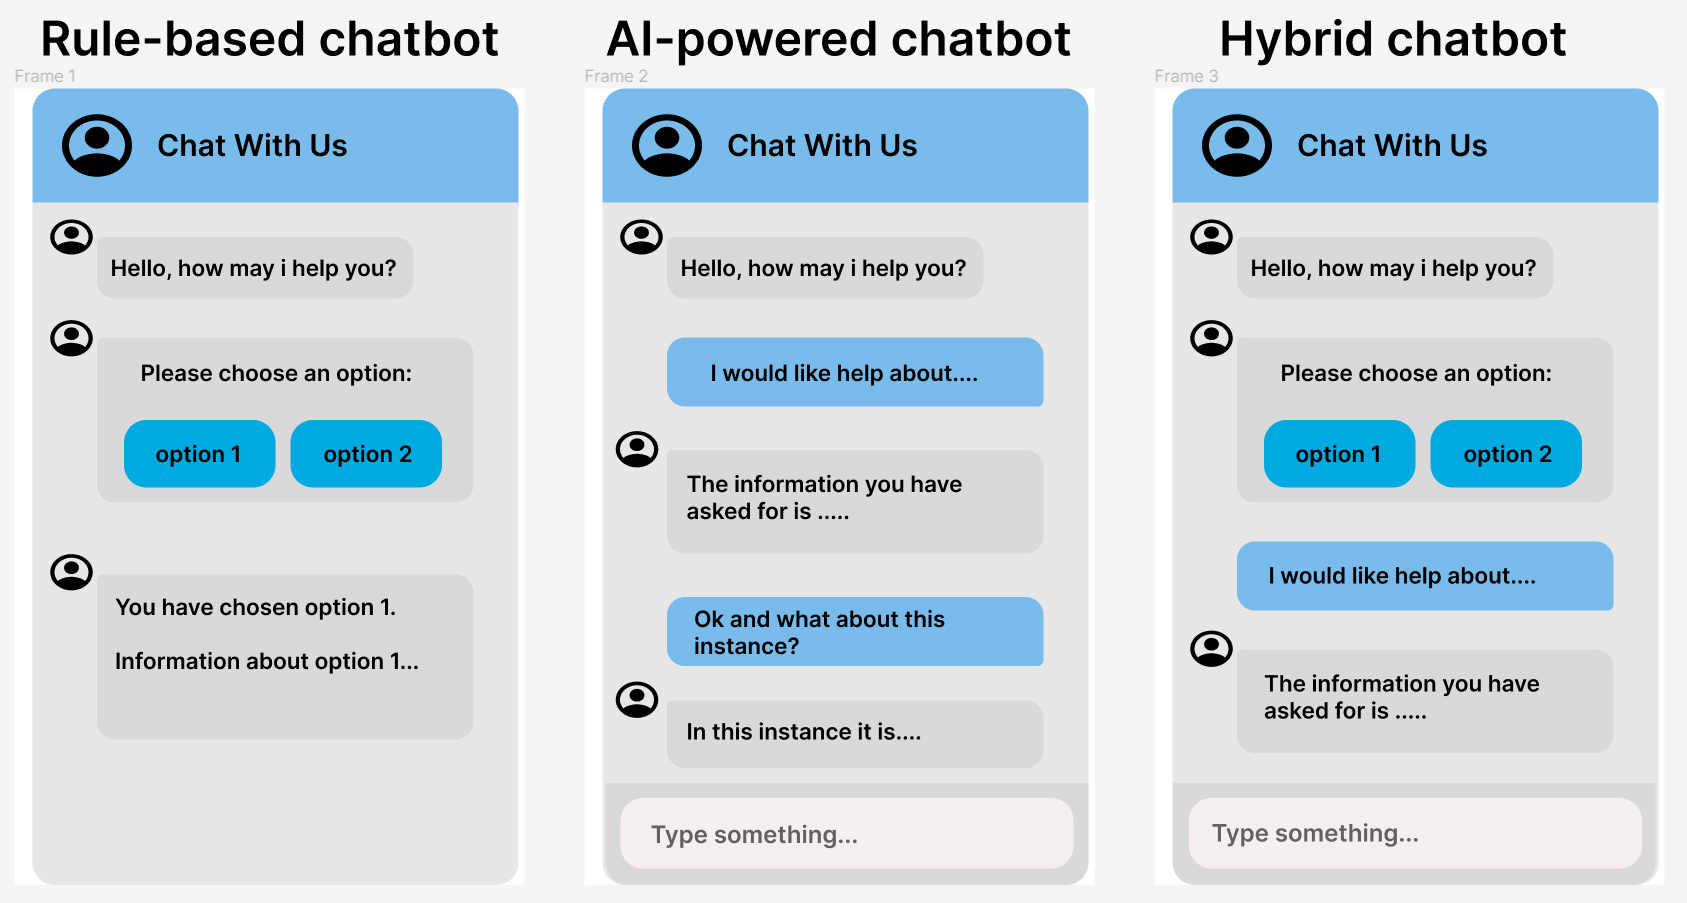
\includegraphics[width=0.75\textwidth]{chatbots}
    \caption{Verschillende soorten chatbots}
    \label{fig:chatbots}
\end{figure}


In de proof-of-concept die zal ontworpen worden zullen we gebruik maken van een Hybride chatbot. De mogelijkheden om snel veel voorkomende vragen te stellen aan de hand van knoppen zal gecombineerd worden met de conversationele kracht van de Large Language Models om specifieke vragen te stellen. De keuze van de Hybride chatbot komt doordat de meeste vragen die binnen komen op de customer service gaan over dezelfde onderwerpen. Aan de hand van sneltoetsen zal het dan mogelijk zijn om deze antwoorden op te halen. Indien er verdere vragen zijn kunnen deze gesteld worden aan de chatbot zelf zoals een conversationele chatbot. 

\section{Hybride chatbot}
Het bouwen van een hybride chatbot in 2023 omvat het combineren van zowel Rule-Based als machine learning gebaseerde benaderingen om een ​​veelzijdig en effectief conversationeel AI-systeem te creëren. Deze chatbots combineren doorgaans Rule-Based systemen met componenten voor machinaal leren en kunstmatige intelligentie om zo een gepersonaliseerd en menselijkere ervaring te creëren. Het doel is om de sterke punten van beide benaderingen te benutten om het beste van beide werelden te bekomen op de applicatie. 

De kernfactoren en belangrijkste attributen van een hybride chatbot zijn~\autocite{Team2023}:

\begin{itemize}
    \item \textbf{Rule-Based componenten:} Deze systemen baseren zich op voorafbepaalde regels en beslissingsstructuren. Ze zijn goed op specifieke opdrachten uit te voeren die een gebruiker bijvoorbeeld meer zou nodig hebben. Een voorbeeld hiervan is enkele vragen die een gebruiker vaak heeft die hij aan de hand van een knop kan vragen in plaats van de vraag volledig uit te typen. 
    \item \textbf{Machine Learning (ML) en Natural Language Processing (NLP):} Machine Learning en Natural Language Processing bestandsdelen geven de chatbot de kracht om menselijke taal te begrijpen en te genereren. Ze hebben het vermogen om de bedoeling van een gebruiker te begrijpen, entiteiten uit een tekst te halen en context te begrijpen. 
    \item \textbf{Intent Recognition:} Intent Recognition is belangrijk om de chatbot het vermogen te geven van het doel van de gebruiker te ontcijferen. Bijvoorbeeld bij de vraag: Wat is het weer morgen? Zal Intent Recognition het doel identificeren als de weersvoorspelling op te halen. 
    \item \textbf{Entity Recognition:} Entity Recognition geeft de chatbot het vermogen van entiteiten/precieze informatie uit de tekst te halen. In het voorbeeld van Intent Recognition over het weer zal het eruit kunnen halen dat de datum 'morgen' is en eventueel een locatie als die wordt meegegeven. 
    \item \textbf{Fallback Mechanisms:} Fallback Mechanismen zijn er eigenlijk als soort van vangnetten voor de chatbot als die een bepaalde query/vraag niet kan behandelen. In dit geval zouden de Fallback Mechanismen er dan voor zorgen dat de chatbot een antwoord kan geven door voorafbepaalde antwoorden op vragen die hij niet kent of kan hij extra vragen stellen om meer informatie te verzamelen. 
\end{itemize}


\section{Semantic Kernel}
Semantic Kernel (SK) is een AI Software Development Kit (SDK) van Microsoft die u de grote taalmogelijkheden van AI-diensten zoals OpenAI naar uw apps brengt~\autocite{Salim}. Het is een open source development kit met nog steeds actieve updates voor verbetering en verschillende programmeertalen te hanteren. Het wordt in de markt gebruikt om applicaties te maken met aan de basis generatieve AI. Developers kunnen aan de hand van deze development kit gemakkelijk de kracht van de AI services te integreren in hun bestaande applicaties. De semantic kernel staat vooral gekend voor zijn vermogen van plannen op te stellen aan de hand waarvan de applicaties dan handelen. Het is in staat van 'plannen' op te stellen om complexe taken uit te voeren zonder de nodige stappen op voorhand al vastgesteld te hebben. Voor complexere applicaties met meerdere prompts voor bepaalde functies zorgt de semantic kernel voor een een programmatie laag aan de hand van semantische functies. Dit zorgt voor een makkelijke scheiding van je C# of python code en je prompts.

\subsection{Planner}
De Semantic kernel is een heel handige development kit om je applicatie de kracht van de  moderne AI modellen te geven en heeft de kracht om zelf de volgorde van de functies te orkestreren. Daarvoor maakt de semantic kernel gebruik van Planners. Een planner is simpelweg een prompt dat zich baseert op de omschrijving van semantische functies om te kiezen welke nodig zijn en in welke volgorde. Deze planners moeten tegenwoordig bijna altijd gebruik maken van het GPT-4 model om goede plannen op te stellen, andere modellen hebben soms moeite met de juiste semantische functies te kiezen~\autocite{Salim}.

\subsection{Semantische functies}
Semantische functies zijn de manier van Semantic Kernel om de LLM prompts na te bootsen. Het grote verschil tussen de LLM prompts en de semantische functies zit hem namelijk in de manier waarop we ze gebruiken. Voor de LLM prompts wordt er vooral gezegd wat er verwacht wordt in grote lijnen en hopen ze dan op de kracht van de LLM om een relevant antwoord te geven, waarbij de semantische functies veel meer in detail over een klein taakje zullen gaan om zo de functies aan elkaar te kunnen koppelen voor een complexere uitkomst gemakkelijk en correct te bekomen. Je kan het dus veel beter sturen van wat je precies als de uitkomst zou willen~\autocite{Salim}. 

\begin{figure}
    \centering
    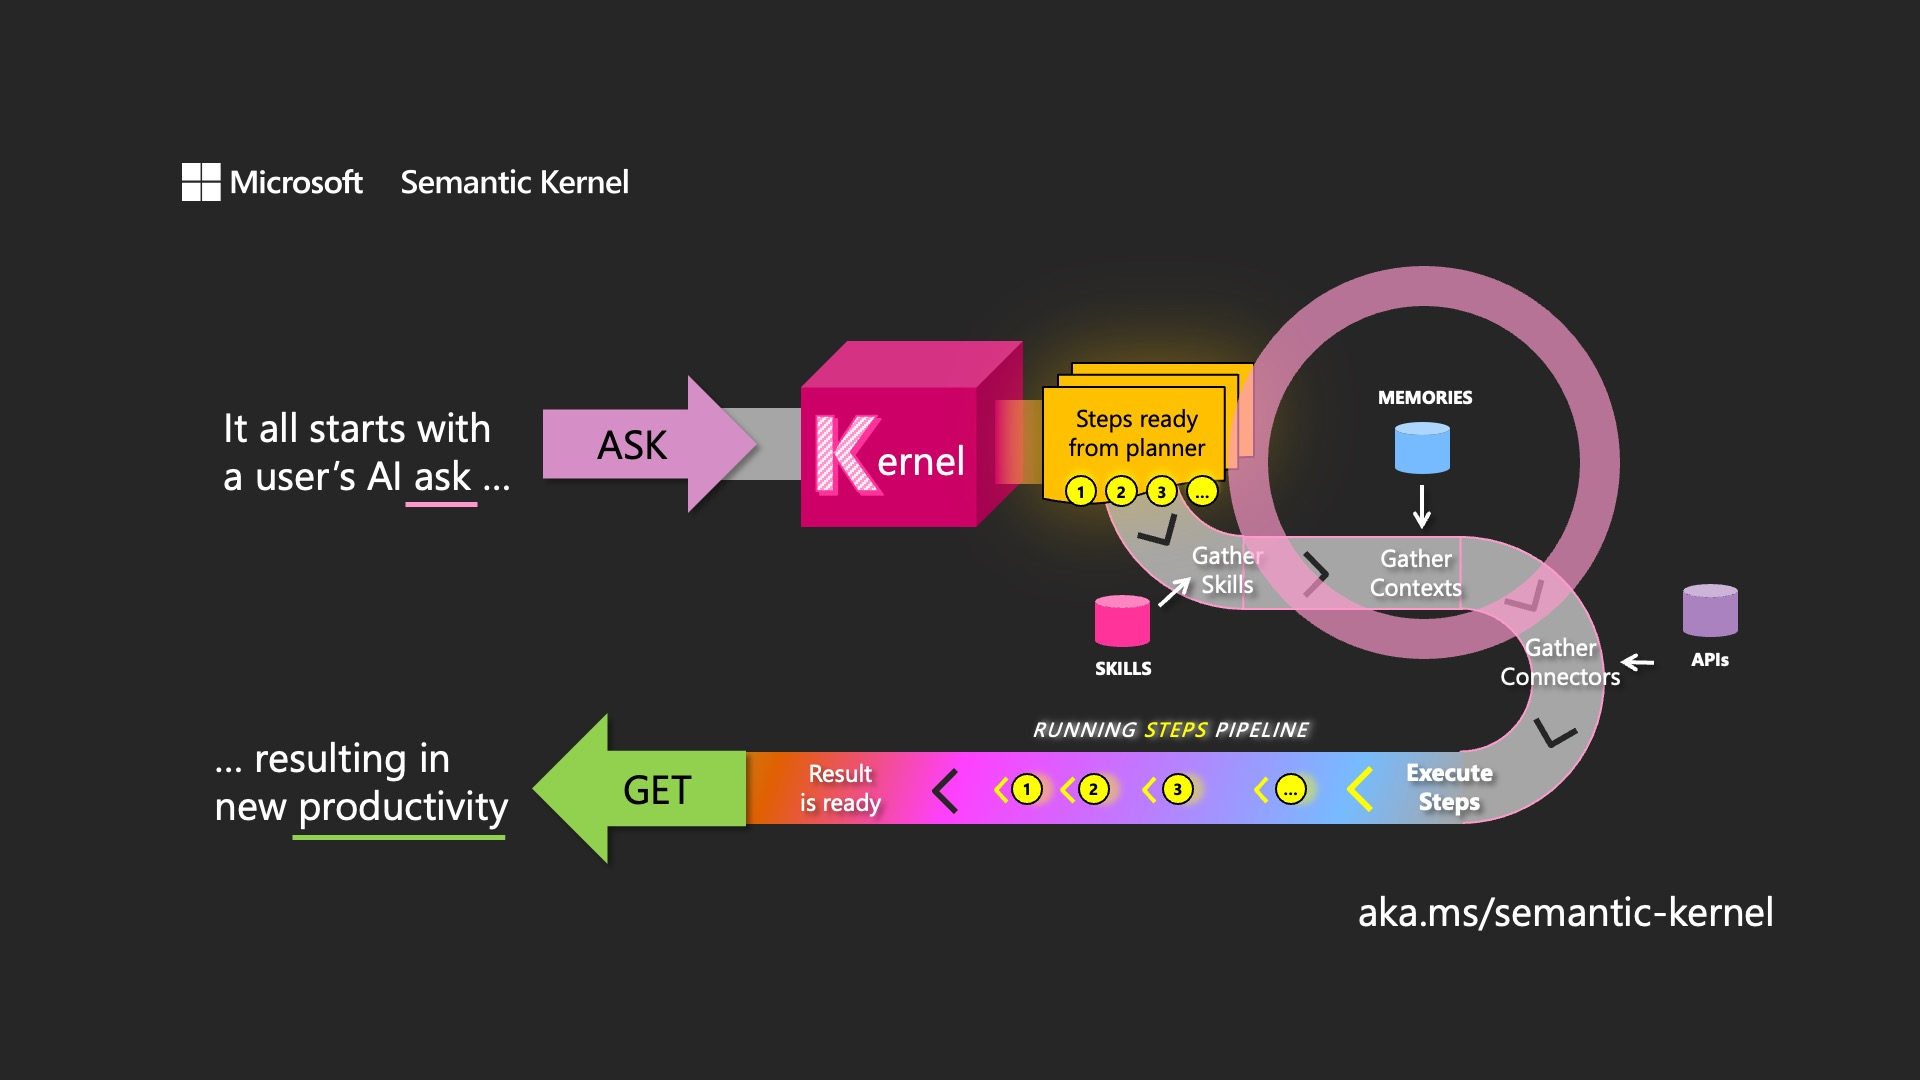
\includegraphics[width=0.75\textwidth]{semantickernel}
    \caption{Het verloop van een vraag met semantic kernel.}
    \label{fig:semanticKernel}
\end{figure}

\subsection{Memory}
Een van de meest voorkomende scenario's bij het bouwen van een AI applicatie is dat je de LLM's moet laten werken met je privé data. De LLM's zijn getrained op grote hoeveelheden publieke data en zullen dus voor taken als een onderwerp van een boek te benoemen of een gebeurtenis in de geschiedenis uitleggen gemakkelijk een antwoord kunnen geven. Bij vragen over privé data zoals een ticket van een klant ophalen zal er wat meer bij moeten komen kijken om de LLM's in staat te stellen van een antwoord te formuleren uit de data.

\subsubsection{Retrieval Augmented Generation (RAG)}
Een veel voorkomende techniek om de mogelijkheid te geven van met privé data te werken is Retrieval Augmented Generation of RAG. Deze techniek is gebaseerd op het combineren van een Search Engine met de LLM's. In deze techniek wordt de LLM gebruikt om het antwoord te genereren terwijl de Search Engine gebruikt wordt om de relevante info uit de privé data te halen~\autocite{Cantina2024}. 
Het hoofddeel van RAG is dus eigenlijk de zoekfunctie. We kunnen ervan uitgaan dat de LLM's goed zijn om menselijke taal te genereren maar dit hangt bij deze techniek heel hard af van welke resultaten de zoekfunctie kan opleveren. Dit wil dus zeggen dat als de zoekfunctie niet goed werkt of de verkeerde info opbrengt zal het antwoord van de LLM ook niet goed zijn. 

\subsubsection{Vector Databases}
Door het probleem dat de zoekfunctie kan ondervinden is er een technologie gevonden die vaak in combinatie kan worden gebruikt met RAG: vector databanken of vector indexen. Het idee van vector databanken is dat ze documenten kunnen opslaan en ophalen aan de hand van de gelijkenis van een vraag. Een van de limitaties van het traditioneel zoeken is dat het gebaseerd is op een sleutelwoord en of het woord aanwezig is in het document of titel. Bij vector databanken kan er gezocht worden op de semantiek van een woord, dit wil zeggen dat er documenten kunnen opgehaald worden dat een samenhangende semantiek hebben met de vraag, ook al bevatten ze niet dezelfde woorden. 
Je kan een vector databank voorstellen als een multidimensionale ruimte waarbij elk document een punt is. De afstand tussen 2 punten is een meetstaaf van hun gelijkaardigheid. Hoe dichter ze bij elkaar liggen hoe meer ze gerelateerd zijn~\autocite{Cantina2024}. 

\begin{figure}
    \centering
    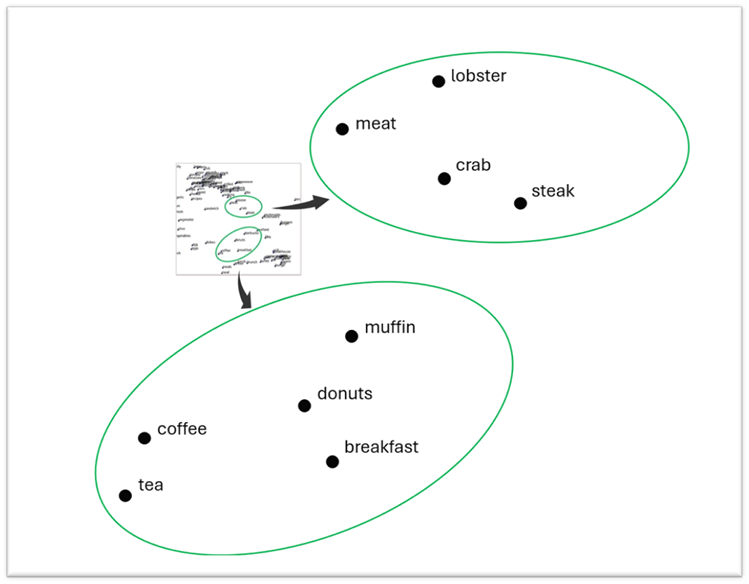
\includegraphics[width=0.75\textwidth]{vectordatabase}
    \caption{Representatie van een vector databank}
    \label{fig:vectordatabase}
\end{figure}

In figuur \ref{fig:vectordatabase} kan je een representatie zien van hoe een vector database opgesteld zou zijn. De punten zijn geen fysieke plaatsen in een databank of computer maar deze punten zijn berekend aan de hand van een wiskundige formule. Zo zie je dat in de ene cirkel een verzameling staat van onderwerpen die te maken hebben met ontbijt en in de andere cirkel gaat het over een grote maaltijd. 

\subsubsection{Kernel Memory}
Kernel Memory gebruikt veel concepten die RAG gebruikt maar dankzij vele extensie functies kan je het gemakkelijk aansluiten aan veelvoorkomende AI diensten (zoals OpenAI en Azure OpenAI) en vector databanken (zoals Azure AI Search). Het wisselen tussen diensten bij Kernel Memory zou geen aanpassing mogen zijn in de code waardoor je dus niet gebonden bent aan een specifieke dienst als developer. Kernel Memory is ook in staat van meerdere types content in embeddings om te zetten. De lange flow om iets op te halen zoals het in de RAG gedaan zou worden is bij Kernel Memory beschikbaar aan de hand van een enkele methode wat de complexiteit veel verminderd~\autocite{Cantina2024}.

Kernel Memory kan op twee manieren werken:

\begin{itemize}
    \item \textbf{Serverless:} De hele dienst wordt rechtstreeks via de applicatie gehost. Dit wil zeggen dat de embeddings worden gegenereerd, opgeslagen en dat de zoekopdracht wordt uitgevoerd binnen de applicatie zelf. Dit is het simpelste scenario maar is niet optimaal voor grote datasets of complexe applicaties doordat het moeilijk te schalen is. 
    \item \textbf{As a service:} De service is gehost als een aparte instantie die de applicatie kan gebruiken aan de hand van een REST API. Dit wordt gezien als de aanbevolen aanpak voor complexe applicaties doordat het je toelaat de dienst onafhankelijk te schalen van de hoofdapplicatie. Zo kan je dit bijvoorbeeld hosten op Azure door gebruik te maken van een App Service om het makkelijk te schalen naar meerdere instanties.
\end{itemize}










%%=============================================================================
%% Methodologie
%%=============================================================================

\chapter{\IfLanguageName{dutch}{Methodologie}{Methodology}}%
\label{ch:methodologie}

%% TODO: In dit hoofstuk geef je een korte toelichting over hoe je te werk bent
%% gegaan. Verdeel je onderzoek in grote fasen, en licht in elke fase toe wat
%% de doelstelling was, welke deliverables daar uit gekomen zijn, en welke
%% onderzoeksmethoden je daarbij toegepast hebt. Verantwoord waarom je
%% op deze manier te werk gegaan bent.
%% 
%% Voorbeelden van zulke fasen zijn: literatuurstudie, opstellen van een
%% requirements-analyse, opstellen long-list (bij vergelijkende studie),
%% selectie van geschikte tools (bij vergelijkende studie, "short-list"),
%% opzetten testopstelling/PoC, uitvoeren testen en verzamelen
%% van resultaten, analyse van resultaten, ...
%%
%% !!!!! LET OP !!!!!
%%
%% Het is uitdrukkelijk NIET de bedoeling dat je het grootste deel van de corpus
%% van je bachelorproef in dit hoofstuk verwerkt! Dit hoofdstuk is eerder een
%% kort overzicht van je plan van aanpak.
%%
%% Maak voor elke fase (behalve het literatuuronderzoek) een NIEUW HOOFDSTUK aan
%% en geef het een gepaste titel.





% Voeg hier je eigen hoofdstukken toe die de ``corpus'' van je bachelorproef
% vormen. De structuur en titels hangen af van je eigen onderzoek. Je kan bv.
% elke fase in je onderzoek in een apart hoofdstuk bespreken.

%\input{...}
%\input{...}
%...

%%=============================================================================
%% Conclusie
%%=============================================================================

\chapter{Conclusie}%
\label{ch:conclusie}

% TODO: Trek een duidelijke conclusie, in de vorm van een antwoord op de
% onderzoeksvra(a)g(en). Wat was jouw bijdrage aan het onderzoeksdomein en
% hoe biedt dit meerwaarde aan het vakgebied/doelgroep? 
% Reflecteer kritisch over het resultaat. In Engelse teksten wordt deze sectie
% ``Discussion'' genoemd. Had je deze uitkomst verwacht? Zijn er zaken die nog
% niet duidelijk zijn?
% Heeft het onderzoek geleid tot nieuwe vragen die uitnodigen tot verder 
%onderzoek?

\lipsum[76-80]



%---------- Bijlagen -----------------------------------------------------------

\appendix

\chapter{Onderzoeksvoorstel}

Het onderwerp van deze bachelorproef is gebaseerd op een onderzoeksvoorstel dat vooraf werd beoordeeld door de promotor. Dat voorstel is opgenomen in deze bijlage.

%% TODO: 
%\section*{Samenvatting}

% Kopieer en plak hier de samenvatting (abstract) van je onderzoeksvoorstel.

% Verwijzing naar het bestand met de inhoud van het onderzoeksvoorstel
%!TEX program = xelatex

\documentclass{hogent-article}

\addbibresource{voorstel.bib}

\studyprogramme{Professionele bachelor toegepaste informatica}
\course{Bachelorproef}
\assignmenttype{Onderzoeksvoorstel}


\academicyear{2023-2024} 


\title{De ontwikkeling van een co-pilot gebaseerd op een MS Dynamics 365 platform}

\author{Arthur Uydens }
\email{arthur.uydens@student.hogent.be}


\supervisor[Co-promotor]{}

\specialisation{Mobile \& Enterprise development}
\keywords{co-pilot, MS Dynamics 365, AI , chatbot}

\begin{document}

\section{Samenvatting}
Dit onderzoeksvoorstel richt zich op het ontwikkelen van een co-pilot op een platform dat gebruik maakt van het MS-Dynamics 365 ERP-pakket.De opdracht is in naam van Itineris waarvan Peter Baeke, R&D Manager Business Unit North America, de rol van co-promotor opneemt en me inhoudelijk zal bijstaan. De co-pilot zou de medewerkers moeten ondersteunen in hun business handelingen en de werkdruk moeten verlagen. Er zal naar zowel het gebruik als naar het correct trainen van de co-pilot gekeken worden om uiteindelijk tot een werkende en efficiënte co-pilot te komen. Er zal onderzocht worden naar de beste manieren waarop de co-pilot gebruikt zal kunnen worden, waar er eventuele valkuilen zitten, hoe de co-pilot getraind kan worden en wat de beste manier is om deze training te voltooien. Met al deze informatie zal er dan een product gemaakt worden om deze opdracht succesvol te voltooien. Met dit eindproduct zullen er verschillende scenario's uitgevoerd worden waarop er dan aan de hand van verschillende criteria beslist wordt of het scenario succesvol is uitgevoerd.

\section{Introductie}
Aritificiële Intelligentie is de wetenschap van de toekomst. Indien je als bedrijf niet op inzet in het jaar 2024 zal je bedrijf een achterstand opwerken op de competitie. Dit onderzoeksvoorstel streeft naar praktische ondersteuning en info te geven over hoe een co-pilot systeem gebruikt kan worden binnen de bestaande applicatie die Itineris aanbied.  

De doelgroep van deze bachelorproef zijn bedrijven die webapplicaties voor andere ondernemingen ontwikkelen. Hier zijn vele voorbeelden van zoals Delaware, HiveCPQ, etc... Deze bedrijven hebben vaak te maken met een grote hoeveelheid gebruikers en data. Het is dus belangrijk dat de applicaties die zij ontwikkelen schaalbaar zijn. Dit betekent dat de applicaties in staat moeten zijn om te groeien en zich aan te passen aan de veranderende behoeften van de gebruikers. Daarnaast moeten de applicaties ook goed presteren en veilig zijn.

De onderzoeksvraag luidt dus: \textbf{
  onderzoeksvraag: Hoe kunnen we de efficiënte ontwikkeling van een co-pilot bevorderen door het identificeren van verschillende valkuilen en trainingsmethoden met specifieke aandacht voor de vereisten van de onderneming? 
}

\section{Doelstellingen}
\begin{enumerate}
  \item Identificeren van de belangrijkste vereisten voor enterprise webapplicaties, met de nadruk op schaalbaarheid, prestaties en beveiliging.
    \begin{itemize}
      \item Welke vereisten zijn het belangrijkst voor de schaalbaarheid van een enterprise webapplicatie?
      \item Welke vereisten zijn het belangrijkst voor de prestaties van een enterprise webapplicatie?
      \item Welke vereisten zijn het belangrijkst voor de beveiliging van een enterprise webapplicatie?
    \end{itemize}
  \item Onderzoeken van best practices in de ontwikkeling van schaalbare webapplicaties en hun toepasbaarheid in een ondernemingsomgeving.
    \begin{itemize}
      \item Wat zijn de best practices voor de ontwikkeling van schaalbare webapplicaties?
      \item Hoe kunnen deze best practices worden toegepast in een ondernemingsomgeving?
      \item Waarom zijn deze best practices belangrijk voor ondernemingen?
    \end{itemize}
  \item Vergelijken van verschillende web development frameworks en technologieën op het gebied van schaalbaarheid, prestaties en onderhoud.
    \begin{itemize}
      \item Wat zijn de meest courante web development frameworks en technologieën?
      \item Waarom worden deze frameworks en technologieën zo veel gebruikt?
    \end{itemize}
  \item Ontwikkelen van een prototype van een schaalbare enterprise webapplicatie en evalueren van de gemaakte keuzes in de ontwikkeling.
\end{enumerate}

\section{Stand van zaken}
Over heel de wereld zijn er al veel bedrijven die schaalbare entreprise webapplicaties maken en dit op een sterke maar ook steeds verschillende manier in stand brengen.

HiveCPQ is de nieuwe leider op de belgische markt in het aanbieden van CPQ-oplossingen aan enterprise-fabrikanten. Je hebt de term CPQ ongetwijfeld al zien voorbijkomen, zeker als je in de maakindustrie werkt. Maar wat is CPQ of Configure-Price-Quote software? CPQ-software helpt bedrijven om hun producten en diensten te configureren, te prijzen en te verkopen. Het is een software die de verkoop van complexe producten en diensten automatiseert en versnelt. CPQ-software is een must voor bedrijven die hun verkoopproces willen optimaliseren en hun omzet willen verhogen. 

Daarnaast hebben we dan ook Delaware, een bedrijf dat begon als een onafhankelijk partnerschap en zich nu heeft uitgewerkt tot een wereldwijde aanwezigheid met meer dan 4600 medewerkers. Delaware is een bedrijf dat geavanceerde ICT-oplossingen en -diensten levert en onze klanten begeleidt bij hun zakelijke en digitale transformaties naar de digitale toekomst.

\section{Methodologie}
\begin{enumerate}
  \item Literatuurstudie: 
  \begin{itemize}
    \item Onderzoek naar bestaande literatuur en documentatie met betrekking tot de ontwikkeling van schaalbare enterprise webapplicaties.
  \end{itemize}
  \item Casestudy's: 
  \begin{itemize}
    \item Analyse van bestaande enterprise webapplicaties om inzicht te krijgen in de gehanteerde methodologieën en technologieën.
  \end{itemize}
  \item Frameworkvergelijking:
  \begin{itemize}
    \item vergelijken van populaire web development frameworks op basis van criteria zoals schaalbaarheid, prestaties en onderhoud.
  \end{itemize}
  \item Prototype-ontwikkeling: 
  \begin{itemize}
    \item Ontwikkeling van een prototype van een schaalbare enterprise webapplicatie, gebruikmakend van de geïdentificeerde best practices en technologieën.
  \end{itemize}
  \item Gebruikerstest:
  \begin{itemize}
    \item Verzamelen van feedback van gebruikers en ontwikkelaars over de ervaringen met het ontwikkelde prototype.
  \end{itemize}
\end{enumerate}

\section{Verwachte resultaten}
\begin{enumerate}
  \item Een overzicht van de belangrijkste vereisten voor schaalbare enterprise webapplicaties.
  \item Identificatie van best practices in de ontwikkeling van schaalbare webapplicaties en hun relevantie voor ondernemingen.
  \item Een vergelijkende analyse van web development frameworks en technologieën op het gebied van schaalbaarheid en prestaties.
  \item Een werkend prototype van een schaalbare enterprise webapplicatie.
\end{enumerate}



\tableofcontents


\end{document}

%%---------- Andere bijlagen --------------------------------------------------
% TODO: Voeg hier eventuele andere bijlagen toe. Bv. als je deze BP voor de
% tweede keer indient, een overzicht van de verbeteringen t.o.v. het origineel.
%\input{...}

%%---------- Backmatter, referentielijst ---------------------------------------

\backmatter{}

\setlength\bibitemsep{2pt} %% Add Some space between the bibliograpy entries
\printbibliography[heading=bibintoc]

\end{document}
